% -*- mode: fundamental -*-

% ****************************************************************

\chapter{RISC-V: the Drum unpipelined CPU (an FSM)}

\markboth{Ch \arabic{chapter}: The Drum CPU code}{\copyrightnotice}

\setcounter{page}{1}
% \renewcommand{\thepage}{\arabic{page}}
\renewcommand{\thepage}{\arabic{chapter}-\arabic{page}}

\label{ch_Drum_code}

% ****************************************************************

\section{Introduction}

In this chapter we use code Drum's behavior, illustrated in
Figure~\ref{Fig_Drum_Instr_Exec}, using BSV's \verb|StmtFSM|
construct to code the FSM.
\begin{figure}[htbp]
  \centerline{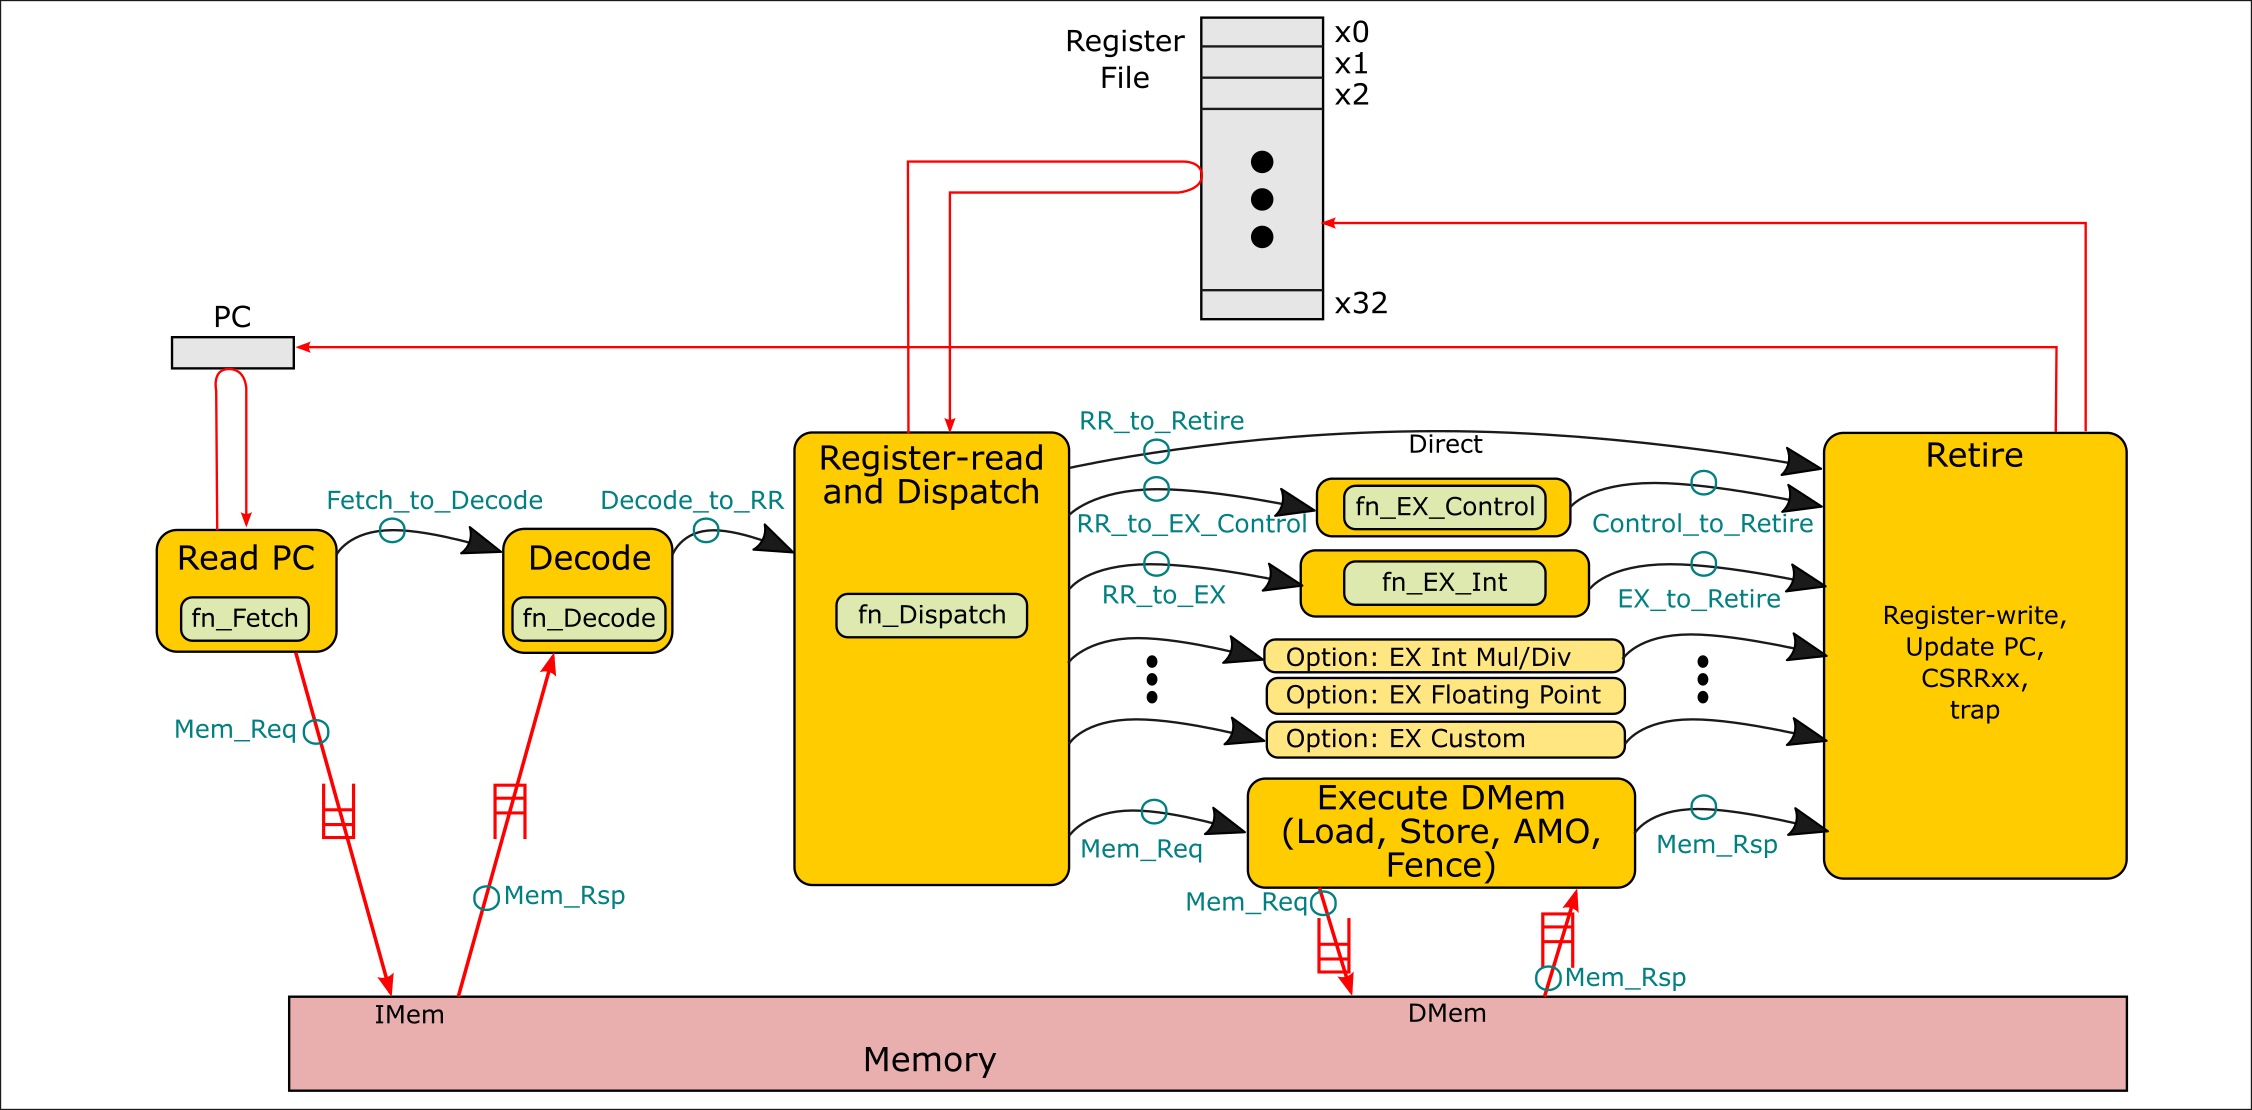
\includegraphics[width=6in,angle=0]{Figures/Fig_Instr_Exec_w_structs}}
  \caption{\label{Fig_Drum_Instr_Exec}
           Simple interpretation of RISC-V instructions
	   (same as Fig.~\ref{Fig_Simple_Instr_Exec_w_structs})}
\end{figure}

% ****************************************************************

\section{The Drum CPU module interface}

\label{Sec_Drum_CPU_interface}

\index[RV]{Drum!CPU interface}

The Drum CPU interface is shown below.

\input{Code_Extracts/CPU_IFC.tex}

The interface is simple:

\begin{tightlist}

  \item The \verb|init| method carries an \verb|Initial_Params| struct
    containing any initial values needed by the CPU.  A typical field
    is the initial value of the PC, since different software systems
    make different assumptions about the ``starting address'' for
    code.  In many RV32I example codes, the starting address is
    \verb|'h_8000_0000|.

  \item A \verb|FIFOF_O| interface to carry memory requests for
    instructions (out-bound from the CPU to the memory);

  \item A \verb|FIFOF_I| interface to carry corresponding memory
    responses containing instructions (in-bound from memory to the
    CPU);

  \item A \verb|FIFO_O| interface to carry memory requests from
    load/store instructions (out-bound from the CPU to the memory);

  \item A \verb|FIFOF_I| interface to carry corresponding load/store
    memory responses (in-bound from memory to the CPU).

\end{tightlist}

(Please re-read Section~\ref{Sec_Harvard_architecture} for the
discussion on Harvard architectures, which have separate memory-access
channels for instructions (Fetch, IMem) and for data (LOAD/STORE,
DMem)).

Later we will see that Fife shares this interface, so that the Fife
and Drum CPUs are easily interchangeable in any system or testbench.

% ****************************************************************

\section{The Drum CPU module}

\label{Sec_Drum_CPU_module}

\index[RV]{Drum!Skeleton module}
\index[RV]{Fife!Skeleton module}

The STATE and INTERFACE sections of the Drum CPU module are shown
below (we will discuss the elided BEHAVIOR section shortly).

\input{Code_Extracts/Drum_mkCPU_STATE.tex}

\hm \emph{(... BEHAVIOR elided, to be discussed shortly ...)}

\input{Code_Extracts/Drum_mkCPU_IFC.tex}

The STATE section first instantiates a register \verb|rg_running|,
initially False, that will be set to True by the \verb|init| method
that initializes the PC to a specific initial value.  The FSM will
wait for this before starting the first instruction-fetch.

Then, \verb|mkCPU| instantiates a register for the PC, and then the
GPRs module (desribed in Section~\ref{Sec_RISCV_regfile}) and the CSRs
modules (described in Section~\ref{Sec_RISCV_CSRs}).  Then, it
instantiates a set of registers to hold values between temporal FSM
steps (with struct types shown in Figure~\ref{Fig_Drum_Instr_Exec}).
For example, the Fetch step will write a value into
\verb|rg_Fetch_to_Decode| which will be read later by the Decode step.
Then, it instantiates four FIFOFs for IMem requests (outgoing) and
responses (incoming), and for DMem requests (outgoing) and responses
(incoming). As mentioned before, we do not make any assumption about
the \emph{latency} of memory requests, {\ie} how long it takes the
external memory subsystem to consume a request from one of the request
FIFOs and enqueue a response into the corresponding response FIFO.
Finally, it instantiates the four registers needed for trap-handling,
described in Section~\ref{Sec_Traps}.

In the display above we have elided the BEHAVIOR section of the
module, which we will describe shortly.

In the INTERFACE section, the \verb|init| method initializes the PC
and sets \verb|rg_running| to true, releasing the BEHAVIOR section to
start executing.  We use the interface transformers discussed in
Section~\ref{Sec_interface_transfomers} that produce Semi-FIFO
``views'' of FIFOs to lift the FIFO interfaces into the module
interface.

% ****************************************************************

\section{Help-functions for the Drum CPU module behavior}

\label{Sec_Drum_FSM_help_fns}

Before we look at the FSM implementing Drum behavior, we first have
some \verb|Action| functions that encapsulate some common actions
performed in several states in the FSM.

% ----------------
\vspace{2ex}

NOTE:
\fbox{\small
\begin{minipage}{5in}

In BSV, function definitions do not have to be at the top-level of a
file, in fact they can be defined at any nested level.  Here, we
define these inside a module.

\end{minipage}}
% ----------------

\vspace{1ex}

The following function writes an rd-value into the the GPRs, in those
cases where the instruction has an rd (\verb|fn_Decode|, described in
Section~\ref{Sec_fn_Decode}, computed \verb|has_rd| for each kind of
instruction):

\input{Code_Extracts/Drum_upd_rd.tex}

The following function is the last action during an instruction's
execution, updating the PC and the instruction number:

\input{Code_Extracts/Drum_redirect.tex}

The following function saves values into registers \verb|rg_epc|,
\verb|rg_cause| and \verb|rg_tval|, when a trap is detected.  These
will later be written into the corresponding CSR registers during
trap-handling.

\input{Code_Extracts/Drum_setup_exc.tex}

% ****************************************************************

\section{The main behavior actions in the Drum CPU module}

\label{Sec_Drum_actions}

\index[RV]{Drum!CPU module actions}

The following sub-sections show the main actions performed by Drum,
corresponding to the components in Figure~\ref{Fig_Drum_Instr_Exec}.

% ----------------
\vspace{2ex}

\index[BSV]{Action@{\tt Action}!as a first-class type}

NOTE:
\fbox{\small
\begin{minipage}{5in}

In BSV, the type {\tt Action} is a first-class type.  This means we
can write ``action expressions'' and bind the result (of type {\tt
Action}) to a name, and then refer to that action later by that name.
We use this capability below first to define the Drum FSM actions;
then we will embed these actions in the Drum FSM in
Section~\ref{Sec_Drum_CPU_module_behavior}.  We also reuse exactly the
same actions in the alternate specification of Drum's behavior using
Rules instead of {\tt StmtFSM} in Chapter~\ref{ch_Drum_Rules}.

\end{minipage}}
% ----------------

% ================================================================

\subsection{FSM action for Fetch}

\input{Code_Extracts/Drum_Fetch.tex}

This action applies \verb|fn_Fetch()| (Section~\ref{Sec_fn_Fetch}) to
the PC, stores the \verb|to_D| part of the result in register
\verb|rg_Fetch_to_Decode|, and sends the \verb|mem_req| part of the
result to the Instruction Memory by enqueueing it on the outgoing
\verb|f_IMem_req| FIFO.  The other end (dequeue end) of the FIFO is in
the module interface.  The outer environment of this module will
dequeue it and forward it to memory.

% ================================================================

\subsection{FSM action for Decode}

\input{Code_Extracts/Drum_Decode.tex}

We pop the response from IMem (bind \verb|mem_rsp| to the value at
head of the FIFO, and also remove it from the FIFO), then apply
\verb|fn_Decode()| (Section~\ref{Sec_fn_Decode}) to the
\verb|Fetch_to_Decode| value from the Fetch step and the IMem
response, and store the function result in register
\verb|rg_Decode_to_RR|.

% ================================================================

\subsection{FSM action for Dispatch}

The next FSM action is the Register-Read and Dispatch step:

\input{Code_Extracts/Drum_RRD.tex}

Using the information in \verb|rg_Decode_to_RR| created in the Decode
step, we read the two registers \verb|rs1| and \verb|rs2|.  We apply
the function \verb|fn_Dispatch| (Section~\ref{Sec_fn_Dispatch}) and
store the result in register \verb|rg_Dispatch|.

Note that we blindly read both registers \verb|rs1| and \verb|rs2|,
even though many instructions do not have one or both of these fields.
In those situations we'll be reading bogus/irrelevant values, but it
does not matter---in the Execute step we will only use these values in
instructions that need them. Recall that while in a software
programming language this may seem unnecessary or wasted work, in this
hardware context nothing is wasted---the hardware for reading both
registers exist, there is nothing lost in using it.

% ================================================================

\subsection{FSM actions for Execute and Retire}

After the Dispatch FSM step, we move on to the Exectute and Retire FSM
steps.  Figure~\ref{Fig_Retire_Drum} shows the details of the four
``flows'' that may follow.
\begin{figure}[htbp]
  \centerline{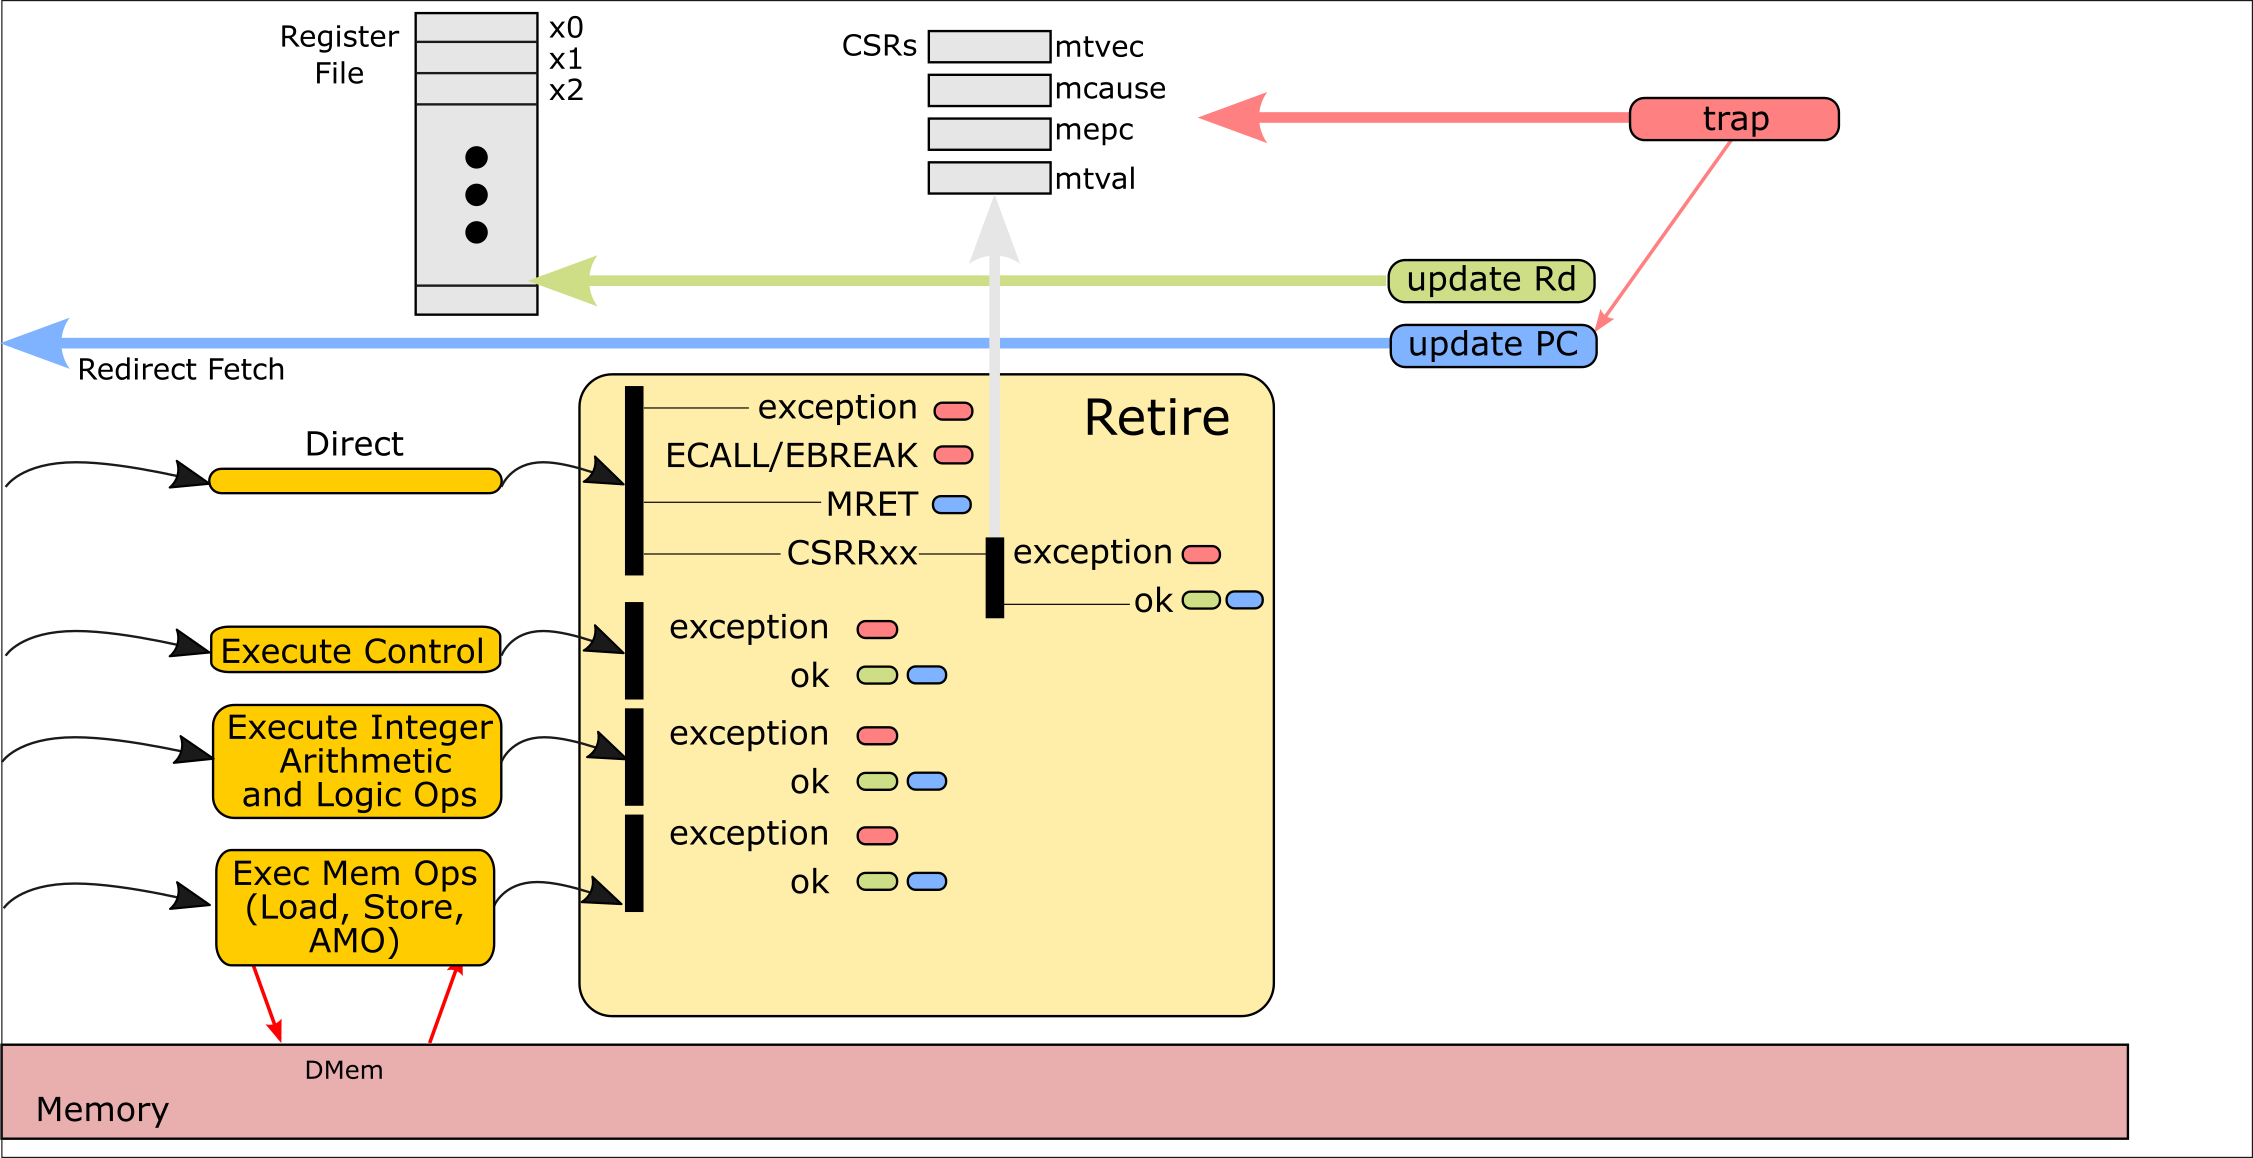
\includegraphics[width=6in,angle=0]{Figures/Fig_Retire_Layers_1}}
  \caption{\label{Fig_Retire_Drum}Execute and Retire actions in Drum}
\end{figure}
Each of the flows can have an exception or a normal (OK) result.  The
Direct flow may need to execute a SYSTEM instruction (ECALL, EBREAK,
MRET and CSRRxx).  Executing a CSRRxx instruction may also have an
exception or normal result.  For each flow, the colored ovals show the
actions may be performed; these correspond exactly to the three
help-functions discussed earlier in Section~\ref{Sec_Drum_FSM_help_fns}.

We next elaborate each of these four flows.

% ----------------------------------------------------------------

\subsubsection{FSM actions in Direct flow of Execute and Retire}

\input{Code_Extracts/Drum_Retire_direct.tex}

First, for convenience, we give the value \verb|rg_Dispatch.to_Retire|
a shorter and more convenient name, \verb|x_direct|, to be used in the
rest of this \verb|action|-\verb|endaction| block.

If we received an exception from the Dispatch step, we invoke the
help-function \verb|fa_setup_exception()|
(Section~\ref{Sec_Drum_FSM_help_fns}) to set register
\verb|rg_exception| to true and to record the relevant values in the
registers \verb|rg_epc|, \verb|rg_epc|, \verb|rg_cause| and
\verb|rg_tval|.

If we received a CSRRxx instruction from the Dispatch step, we invoke
the \verb|mav_csrrxx()| method in the \verb|csrs| module to perform
the instruction on the relevant CSRs.  The result is a 2-tuple
(Section~\ref{Sec_Tuples}) and we use a \verb|match| construct bind
the names \verb|exc| and \verb|rd_val| to the two components.  If the
CSRRxx instruction failed (\verb|exc| is true), once again we invoke
\verb|fa_setup_exception()| to record this.  Otherwise, we invoke
\verb|fa_update_rd()| to write \verb|rd_val| to a GPR, and we invoke
\verb|fa_redirect_Fetch()| to update the PC to the fall-through PC
value.

If we received an MRET instruction from the Dispatch step, we simply
invoke \verb|fa_redirect_Fetch()| to resume executing at the PC value
provided in \verb|rg_mtvec|.

If we received an ECALL or EBREAK instruction from the Dispatch step,
recall from Section~\ref{Sec_ECALL_EBREAK} that these instructions
merely invoke exceptions, with ``cause codes''
\verb|cause_ECALL_FROM_M| and \verb|cause_BREAKPOINT|, respectively
(Section~\ref{Sec_Traps} discussed cause codes).  We simply invoke
\verb|fa_setup_exception()| to record this.  Inside this clause, since
we are already assured that the current insruction is either ECALL or
EBREAK, we only need to check one bit (\verb|instr[20]|) to
distinguish them in order to select the correct cause code.

There is a final ``\verb|else|'' clause, but between the functionality
of the Decode and Dispatch steps, it should be impossible to enter
this clause (this is just a bit of defensive programming and can
safely be removed; even if not removed, it does not produce any
hardware).

% ----------------------------------------------------------------

\subsubsection{Counting retired instructions in CSR {\tt minstret}}

The RISC-V specification says that there is a CSR called
\verb|minstret| that keeps a count of all retired instructions.  This
is often used for performance measurement; for example \verb|minstret|
divided by time gives us a measure of CPU speed,
``instructions/second''.

There are only two nuances for which we must take special care.
First, any instruction that raises an exception is considered to be
``not retired'', so we do not increment \verb|minstret| in that case.

Second, suppose \verb|minstret| has the value 1000, and the next
instruction we retire is a CSRRxx instruction that writes 600 into CSR
\verb|minstret|.  Should the final value of \verb|minstret| be 1001?
Or 600? Or 601? Or something else?  The RISV-V spec says it should be
600, {\ie} an explicit CSRRxx write into \verb|minstret| should
override any implicit increment of the CSR.

In the Drum code, we invoke:

{\small
\begin{Verbatim}
   csrs.ma_incr_instret;
\end{Verbatim}
}

to increment \verb|minstret| inside the \verb|csrs| module in almost
all cases:

\hmm
\begin{tabular}{ll}
 in {\tt a\_Retire\_direct}   & for MRET, ECALL and EBREAK but not for CSRRxx \\
 in {\tt a\_Retire\_Int}      & when not an exception \\
 in {\tt a\_Retire\_Control}  & when not an exception \\
 in {\tt a\_Retire\_DMem}     & when not an exception
\end{tabular}

In the remaining case for {\tt a\_Retire\_direct}, CSRRxx, we invoke
this method---{\tt csrs.mav\_csrrxx()}---which performs the CSRRxx
instruction, and increments \verb|minstret| if there is no exception
and if it did not write to CSR \verb|minstret|.

% ----------------------------------------------------------------

\subsubsection{FSM actions in Execute and Retire Control flow}

The Control path is a sequence of two actions.  First, we have an
Execute action invokes \verb|fn_EX_Control|
(Section~\ref{Sec_fn_EX_Control}) on the information provided by
Dispatch, and stores the result in register
\verb|rg_EX_Control_to_Retire|:

\input{Code_Extracts/Drum_EX_Control.tex}

Then, the Retire action checks if Execute resulted in an exception or
not. If an exception, it invokes \verb|fa_setup_exception| to record
that.  If not an exception, it invokes \verb|fa_update_rd| to store
the output value (this can only be a ``return address'' computed for
JAL and JALR), and it invokes \verb|fa_redirect_Fetch| to resume
execution at the \verb|next_pc| value computed by BRANCH/JAL/JALR.

\input{Code_Extracts/Drum_Retire_Control.tex}

% ----------------------------------------------------------------

\subsubsection{FSM actions in Execute and Retire Integer flow}

This sub-FSM is similar to the Control sub-FSM: it is also a sequence
of two actions.  The Execute action invokes \verb|fn_EX_Int|
(Section~\ref{Sec_fn_EX_Int}) on the information provided by Dispatch,
and stores the result in register \verb|rg_EX_to_Retire|.

\input{Code_Extracts/Drum_EX_Int.tex}

Then, the Retire action checks if Execute resulted in an exception or
not. If an exception, it invokes \verb|fa_setup_exception| to record
that.  If not an exception, it invokes \verb|fa_update_rd| to store
the output value and \verb|fa_redirect_Fetch| to resume execution at
the fall-through PC.

\input{Code_Extracts/Drum_Retire_Int.tex}

% ----------------------------------------------------------------

\subsubsection{FSM actions in Execute and Retire DMem flow}

This sub-FSM is similar to Control and Integers sub-FSMs: it is also a
sequence of two actions.  The Execute action just sends the
memory-request provided by the Dispatch stage to memory by enqueueing
it on the outgoing \verb|f_DMem_req| FIFO.

\input{Code_Extracts/Drum_EX_DMem.tex}

Then, the Retire action pops the mememory response from the incoming
\verb|f_DMem_rsp| FIFO.  If the memory returned an exception, we
compute the proper cause code and then invoke
\verb|fa_setup_exception()| to record it.  If the memory did not
return an exception, we invoke \verb|fa_update_rd()| to store any
loaded value into the GPRs, and invoke \verb|fa_redirect_Fetch()| to
resume execution at the fall-through PC.

\input{Code_Extracts/Drum_Retire_DMem.tex}

% ----------------------------------------------------------------

\subsection{FSM actions for exceptions}

The final action of the Drum FSM is used in case any of the Retire
flows recorded an exception.  It invokes the \verb|mav_exception()|
method in the CSRs module, and invokes \verb|fa_redirect_Fetch| so
that execution resumes at the trap-vector PC provided in CSR
\verb|mt_vec|.

\input{Code_Extracts/Drum_exc.tex}

% ****************************************************************

\section{The Drum CPU module behavior}

\label{Sec_Drum_CPU_module_behavior}

\index[RV]{Drum!CPU module behavior}

Having defined all the actions needed by Drum, we can now assemble
them into the Drum FSM.  First we define an FSM specification
\verb|exec_one_instr| (of type \verb|Stmt|) for executing a single
instruction.

Then, we embed that \verb|Stmt| in a next-level
\verb|Stmt| in an infinite while-loop, preceded by an \verb|await|
action that waits for the initial PC to be set by the \verb|init|
method. Finally, we instantiate that \verb|Stmt| using a
\verb|mkAutoFSM| module that will implement the behavior starting
immediately when the circuit emerges from reset.  The FSM never stops,
because of the infinite while-loop.

{\small
\begin{Verbatim}
module mkCPU (CPU_IFC);
   // STATE
   ...
   // ****************************************************************
   // BEHAVIOR
   ...
\end{Verbatim}
}

\input{Code_Extracts/Drum_exec_one_instr.tex}
\input{Code_Extracts/Drum_FSM.tex}

{\small
\begin{Verbatim}
   // ****************************************************************
   // INTERFACE
   ...
endmodule
\end{Verbatim}
}

Recall that each \verb|Action| is instantaneous, and that FSMs
sequence actions.  In the FSM, the Fetch action \verb|a_Fetch| takes
place in one instant; the Decode action \verb|a_Decode| takes place at
a later instant; the \verb|a_Register_Read_and_Dispatch| action takes
place at an even later instant.  After that, the FSM goes down one of
four alternative paths (Direct, Control, Int and DMem).  Finally, if
\verb|rg_exception| is true, it performs \verb|a_exception|.

The \verb|a_Fetch| action tries to enqueue an IMem request to memory
and enqueue an \verb|Fetch_to_Decode| struct on an output FIFO.  The
action is not ``enabled'' until both FIFOs have space available (are
not full).  When the Fetch action fires, both enqueues are performed,
atomically.

The \verb|a_Decode| action tries to dequeue an IMem response from
memory, dequeue a \verb|Fetch_to_Decode| struct from an imput FIFO,
and enqueue a \verb|Decode_to_RR| struct on an output FIFO.  The
action is not ``enabled'' until the input FIFOs have data available
(are not empty) and the output FIFO has space available (is not full).
When the Decode action fires, both dequeues and an the enqueue are
performed, atomically.

Thus, the time interval between the Fetch instant and the Decode
instant is unpredictable; it depends on when input FIFOs are not empty
and output FIFOs are not full (see dicussion in
Section~\ref{Sec_mem_latency} on unpredictable memory latency).

% ----------------
\vspace{2ex}

NOTE:
\fbox{\small
\begin{minipage}{5in}

Looking ahead to a topic we'll discuss in more detail in
Chapter~\ref{ch_Rules_I}, each module interface method has a so-called
\emph{implicit condition}, {\ie} an accompanying boolean value value
that indicates when the method is READY or not or, to say it another
way, whether the method is ENABLED or not.  For the FIFO methods
``{\tt .first}'' and ``{\tt .deq}'', which are used by ``{\tt
pop\_o}'' above, the methods are ready/enabled only when the FIFO is
not empty.  The ``{\tt enq}'' method is ready/enabled only when the
FIFO is not full.

\vspace{1ex}

The Decode action in the FSM is translated by the \emph{bsc} compiler
into a BSV \emph{rule}.  A rule does not ``fire'' until all the
implicit conditions in its method-calls are enabled.  This is why the
Decode action implicitly waits until something is available in the
FIFO.

\end{minipage}}
% ----------------

% ----------------
\hdivider

\Exercise

What might happen if we omitted the ``{\tt await!(rg\_running)}''
statement in the Drum CPU? (Try it in simulation!)

\emph{Hint:} The FSM may start running before the PC has been initialized ...

\Endexercise
% ----------------

% ****************************************************************

\section{Conclusion}

And that is the complete Drum CPU!  We can compile it with \emph{bsc}
into Verilog, connect the CPU interface to a memory system, and run
the system to execute RISC-V programs compiled for the RV32I ISA
subset (and, further, Drum can recover from illegal instructions due
to trap-handling).

% ================================================================

\subsection{But Drum code looks just like C!?  Why not code it in C?}

Looking at the BSV FSM code for Drum, it seems like we could convert
it into C code by simply replacing a few BSV idioms with corresponding
C idioms (like replacing {\tt begin}-{\tt end} and {\tt action}-{\tt
endaction} with ``{\tt \{}'' and ``{\tt \}}'', replacing BSV register
declarations with C variable declarations, {\etc}).  Similarly, each
of the pure functions {\tt fn\_Fetch}, {\tt fn\_Decode}, ...  can
easily be slightly tweaked into C functions.

This can indeed be done, and the result would be a C simulator for
RISC-V!  We could compile it with any C compiler and run the software
on any platform.

So, why not code Drum in C instead of BSV, and change the \emph{bsc}
compiler to accept C syntax?  It is difficult to compile
general-purpose C into hardware.  C has many constructs that have no
obvious mapping into hardware, such as pointers, the address-of
operator ``\verb|&|'', address arithmetic, \verb|malloc|, and so on.
But can't we define a restricted subset of C suitable for hardware
design?  Compilation is still very difficult.  In the suggested
re-coding in C above, we lose the distinction between variables used
to hold state (registers, register files, FIFOs) and ordinary
variables for temporary values (which in hardware are just wires).  We
also lose the distinction between non-temporal statements (statements
within an action block) versus temporally sequenced (actions in an
FSM).  A C-to-hardware compiler would have to reconstruct this
information.

But the killer reason is sequentiality {\vs} concurrency.  With Drum
it is deceptively easy to imagine a simple correspondence with C,
because Drum is a sequential FSM, and C is a sequential language.
When we advance to concurrent FSMs, including pipelined processors
like Fife, we depart subtantially and deeply from sequential process
semantics, and C becomes more and more unsuitable for hardware
description.

% ----------------
\vspace{2ex}

NOTE:
\fbox{\small
\begin{minipage}{5in}

There are products in the marketplace under the rubric of ``High Level
Synthesis'' (HLS) that translate C source codes into synthesizable
Verilog.  These indeed work on a carefully defined subset of C, not
the full C language.  They work best on simple programs that contain
nested loops working on dense, rectangular arrays (many
image-processing and linear algebra applications can be so
characterized), because the compiler is able to analyze the originally
sequential semantics of such programs and transform them into highly
parallel, highly structured representations that can then be mapped
into very stylized hardware (data path plus control FSM).  Even with
this capability, the programmer may need to provide many additional
directives to the compiler to guide it towards good quality hardware.
We do not consider this to be a general purpose approach to hardware
design.

\vspace{1ex}

See also Appendix~\ref{apx_Why_BSV} for more discussion on this topic.

\end{minipage}}
% ----------------

% ****************************************************************
